\documentclass[a4paper,12pt]{article}

\usepackage[utf8]{inputenc}
\usepackage[spanish]{babel}
\usepackage{amsmath, amssymb}
\usepackage{graphicx}
\usepackage{float}
\usepackage{booktabs}
\usepackage{xcolor}
\usepackage{listings}
\usepackage{caption}
\usepackage{fancyhdr}
\usepackage{hyperref}
\usepackage{tikz}

\hypersetup{
    colorlinks=true,
    linkcolor=blue,
    urlcolor=blue,
    pdftitle={Práctica 1 - ESP32},
}

% ---------- PREÁMBULO: arreglar comillas en listings (Thonny style) ----------
\usepackage[utf8]{inputenc}   % si no está ya
\usepackage[T1]{fontenc}      % mejor soporte de tipografías para PDFs
\usepackage{textcomp}         % símbolos de texto adicionales
\usepackage{upquote}          % comillas ' y " tipo ASCII en verbatim/listings

% Si usas babel con español, desactiva el shorthand de la comilla doble
\usepackage[spanish]{babel}
\shorthandoff{"}  % <<< evita que " sea un caracter activo (causa comillas invisibles)

% Colores inspirados en Thonny
\usepackage{xcolor}
\definecolor{thonnyKeyword}{rgb}{0.0,0.2,0.8}
\definecolor{thonnyComment}{rgb}{0.0,0.5,0.0}
\definecolor{thonnyString}{rgb}{0.7,0.12,0.12}
\definecolor{thonnyBackground}{rgb}{1.0,1.0,1.0}
\definecolor{thonnyBuiltin}{rgb}{0.5,0.0,0.5}
\definecolor{thonnyNumber}{rgb}{0.35,0.35,0.35}

% Declaración de lenguaje MicroPython (basado en Python)
\usepackage{listings}
\lstdefinelanguage{MicroPython}{
    morekeywords={
        False, True, None, and, as, assert, async, await, break, class, continue,
        def, del, elif, else, except, finally, for, from, global, if, import,
        in, is, lambda, nonlocal, not, or, pass, raise, return, try, while, with, yield
    },
    morekeywords=[2]{print,open,range,len,abs,int,float,str,dict,list,set,tuple},
    morekeywords=[3]{machine,network,time,urequests,utime,gc,Pin,ADC,PWM,UART,RTC,ESP32},
    sensitive=true,
    morecomment=[l]{\#},
    morestring=[b]",
    morestring=[b]',
}

% Configuración de listings con estilo Thonny (y upquote activo)
\lstset{
    language=MicroPython,
    backgroundcolor=\color{thonnyBackground},
    keywordstyle=\color{thonnyKeyword}\bfseries,
    keywordstyle=[2]\color{thonnyBuiltin},
    keywordstyle=[3]\color{thonnyKeyword!60!black},
    commentstyle=\color{thonnyComment}\itshape,
    stringstyle=\color{thonnyString},
    numberstyle=\tiny\color{thonnyNumber},
    basicstyle=\ttfamily\small,
    numbers=left,
    numbersep=6pt,
    frame=single,
    framerule=0.4pt,
    breaklines=true,
    breakatwhitespace=true,
    showstringspaces=false,
    tabsize=2,
    captionpos=b,
    columns=flexible,
    upquote=true     % importante para mostrar comillas rectas correctamente
}

\title{Práctica N°1: Inicializacion de OLED y perifericos en PIC32 MAX32}
\date{}

\begin{document}
\maketitle
\tableofcontents
\newpage

\section{Objetivos}

\subsection{Objetivo general}
\begin{itemize}
  \item Diseñar, implementar y documentar una guía práctica que permita a un estudiante instalar y usar PlatformIO en Visual Studio Code para programar una matriz LED 16\(\times\)16 basada en WS2812 con un ESP32, de modo que pueda desplegar efectos visuales (rainbow, plasma, fuegos artificiales, tablero ajedrez) y texto desplazable con funcionamiento seguro y reproducible.
\end{itemize}

\subsection{Objetivos específicos}
\begin{enumerate}
  \item \textbf{Instalación del entorno:} Mostrar paso a paso la instalación de Visual Studio Code y la extensión PlatformIO, crear un proyecto nuevo para ESP32 y verificar la conexión entre la placa y PlatformIO (compilación y carga de un sketch de prueba).
  \item \textbf{Gestión de dependencias:} Incluir las instrucciones para agregar la librería \texttt{FastLED} en \texttt{platformio.ini} y verificar su correcto funcionamiento mediante un ejemplo mínimo.
  \item \textbf{Portado y explicación del código:} Incluir el código proporcionado (mapeo XY serpentina, fuente 5x7, efectos y scroll) con explicaciones linea-por-línea de las partes críticas: inicialización de FastLED, \texttt{XY()}, ISR del botón, y gestión de modos.
  \item \textbf{Pruebas en hardware:} Definir procedimientos de prueba (lista de verificación) para comprobar el mapeo, la orientación de la matriz, el brillo seguro y la respuesta del botón (debounce). Incluir criterios de aceptación (por ejemplo: todas las filas/columnas deben encenderse correctamente con el patrón de test; el cambio de modo debe ser estable y reproducible).
\end{enumerate}

\section{Instalación del entorno de desarrollo}

En esta sección se detallan los pasos necesarios para preparar el entorno de desarrollo basado en \textbf{Visual Studio Code (VSCode)} con la extensión \textbf{PlatformIO}, que permite programar el microcontrolador \textbf{ESP32} de forma profesional, integrando herramientas de compilación, carga y gestión de librerías.

\subsection{Instalación de Visual Studio Code}

\begin{enumerate}
  \item Acceder al sitio oficial de descarga: \url{https://code.visualstudio.com/}.
  \item Descargar la versión correspondiente al sistema operativo Windows.
  \item Ejecutar el instalador y seguir los pasos del asistente, dejando activadas las opciones recomendadas.
\end{enumerate}


Una vez completada la instalación, abrir VSCode para verificar que la interfaz inicial se muestra correctamente.

\subsection{Instalación de la extensión PlatformIO IDE}

\begin{enumerate}
  \item En la barra lateral izquierda de VSCode, hacer clic en el icono de \textbf{Extensiones}.
  \item En la barra de búsqueda escribir: \texttt{PlatformIO IDE}.
  \item Seleccionar la extensión oficial de \textbf{PlatformIO Labs LLC}.
  \item Pulsar en el botón \textbf{Install}.
\end{enumerate}

\begin{figure}[H]
  \centering
  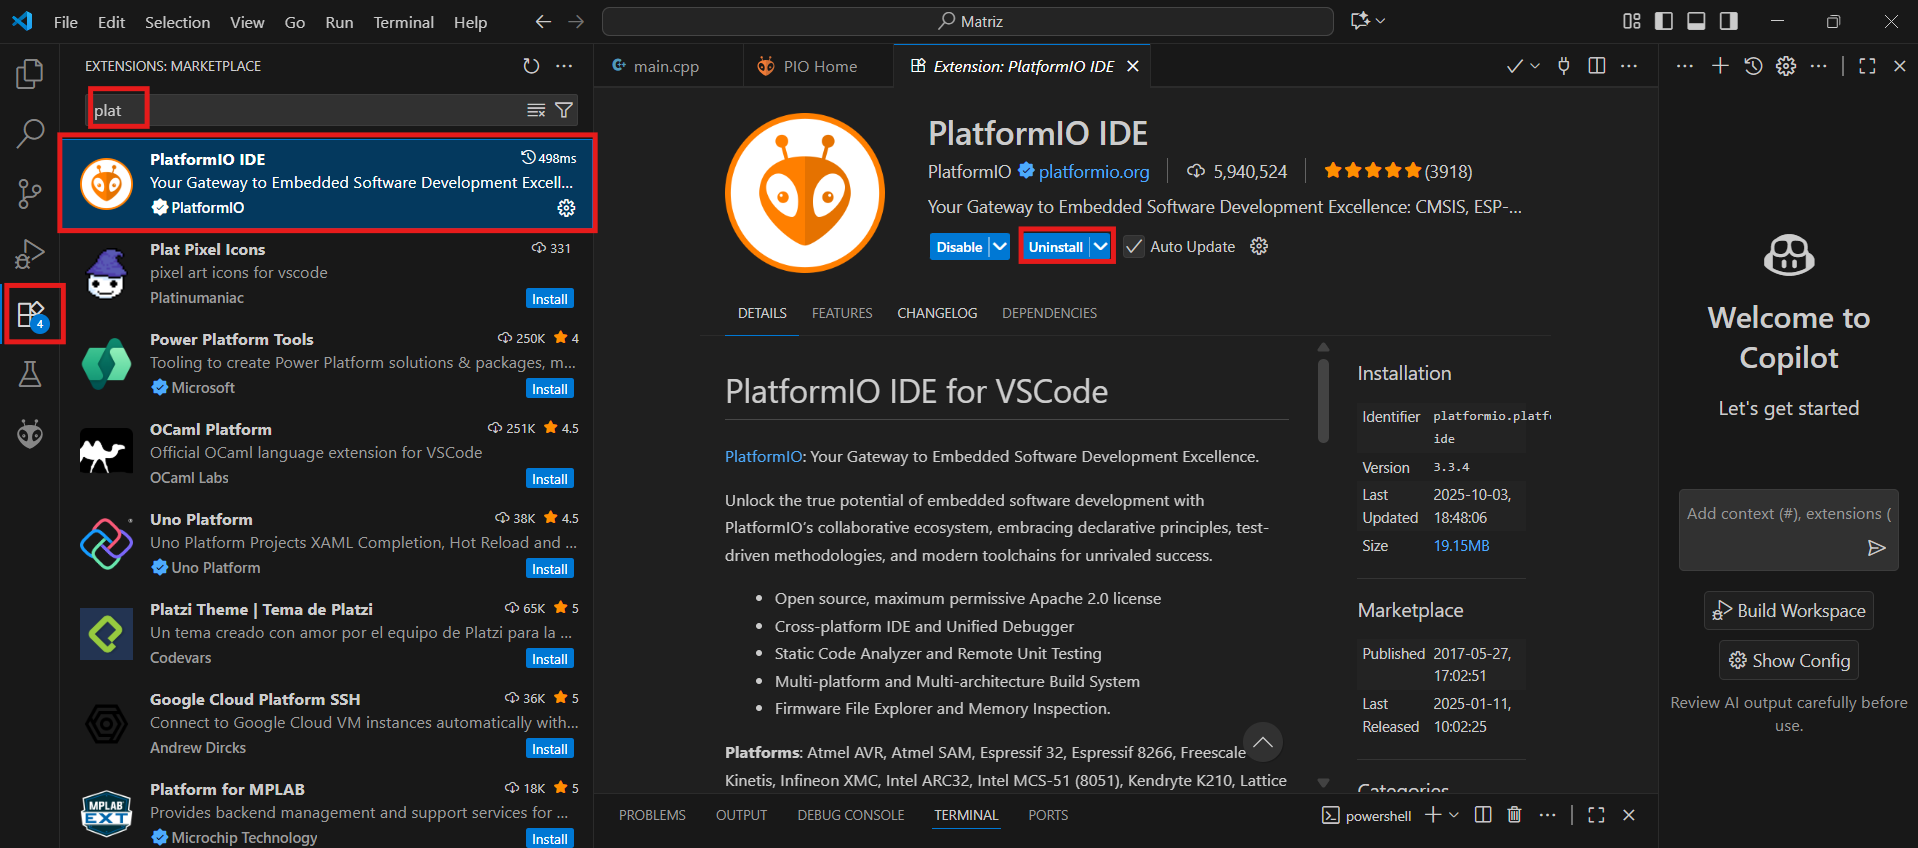
\includegraphics[width=0.75\textwidth]{Platformio/instalacion_plat.png}
  \caption{Instalación de la extensión PlatformIO IDE desde el marketplace de VSCode.}
\end{figure}

Tras la instalación, PlatformIO añadirá un icono con el logotipo del “hormiga” (\textbf{ant}) en la barra lateral izquierda. Al hacer clic sobre él se accede al panel de control principal.

\subsection{Creación de un nuevo proyecto para ESP32}

\begin{enumerate}
  \item En el menú lateral de PlatformIO, seleccionar \textbf{New Project}.
  \item Asignar un nombre al proyecto (por ejemplo: \texttt{Matriz\_LED\_ESP32}).
  \item En \textbf{Board}, seleccionar la placa utilizada, por ejemplo \texttt{ESP32 Dev Module}.
  \item En \textbf{Framework}, elegir \texttt{Arduino}.
  \item Pulsar \textbf{Finish} y esperar a que PlatformIO configure automáticamente la estructura del proyecto.
\end{enumerate}

\begin{figure}[H]
  \centering
  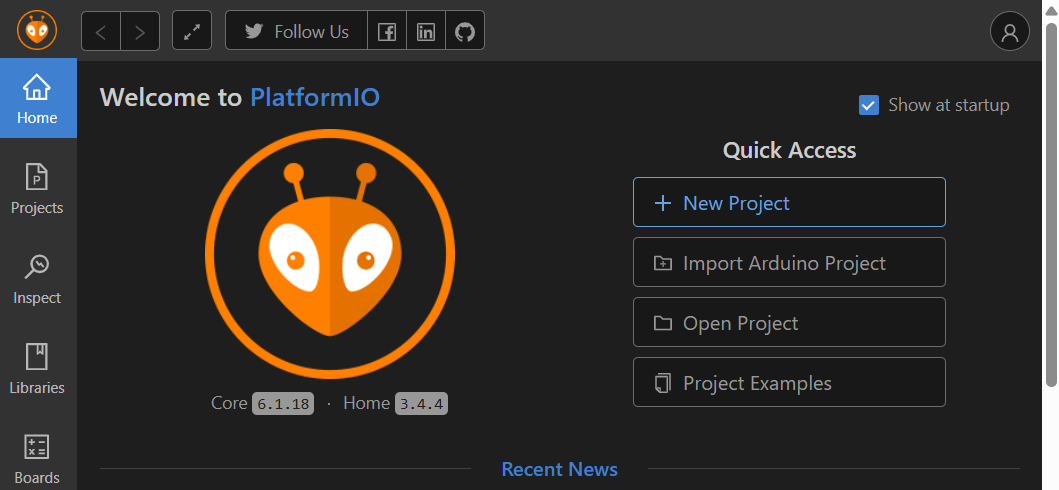
\includegraphics[width=0.75\textwidth]{Platformio/crear_proyecto.png}
  \caption{Creación de un nuevo proyecto en PlatformIO para ESP32 con el framework Arduino.}
\end{figure}

\subsection{Instalación de la librería \texttt{FastLED}}

La librería \texttt{FastLED} es necesaria para controlar las matrices de LED direccionables como las WS2812. Existen dos métodos para instalarla: usando la interfaz de PlatformIO o editando el archivo de configuración.

\subsubsection{Método 1: desde el gestor de librerías de PlatformIO}

\begin{enumerate}
  \item Hacer clic en el icono de PlatformIO (barra lateral izquierda).
  \item Seleccionar la pestaña \textbf{Libraries}.
  \item Escribir en el buscador: \texttt{FastLED}.
  \item Seleccionar la librería oficial de \textbf{Daniel Garcia}.
  \item Pulsar \textbf{Install}.
\end{enumerate}

\begin{figure}[H]
  \centering
  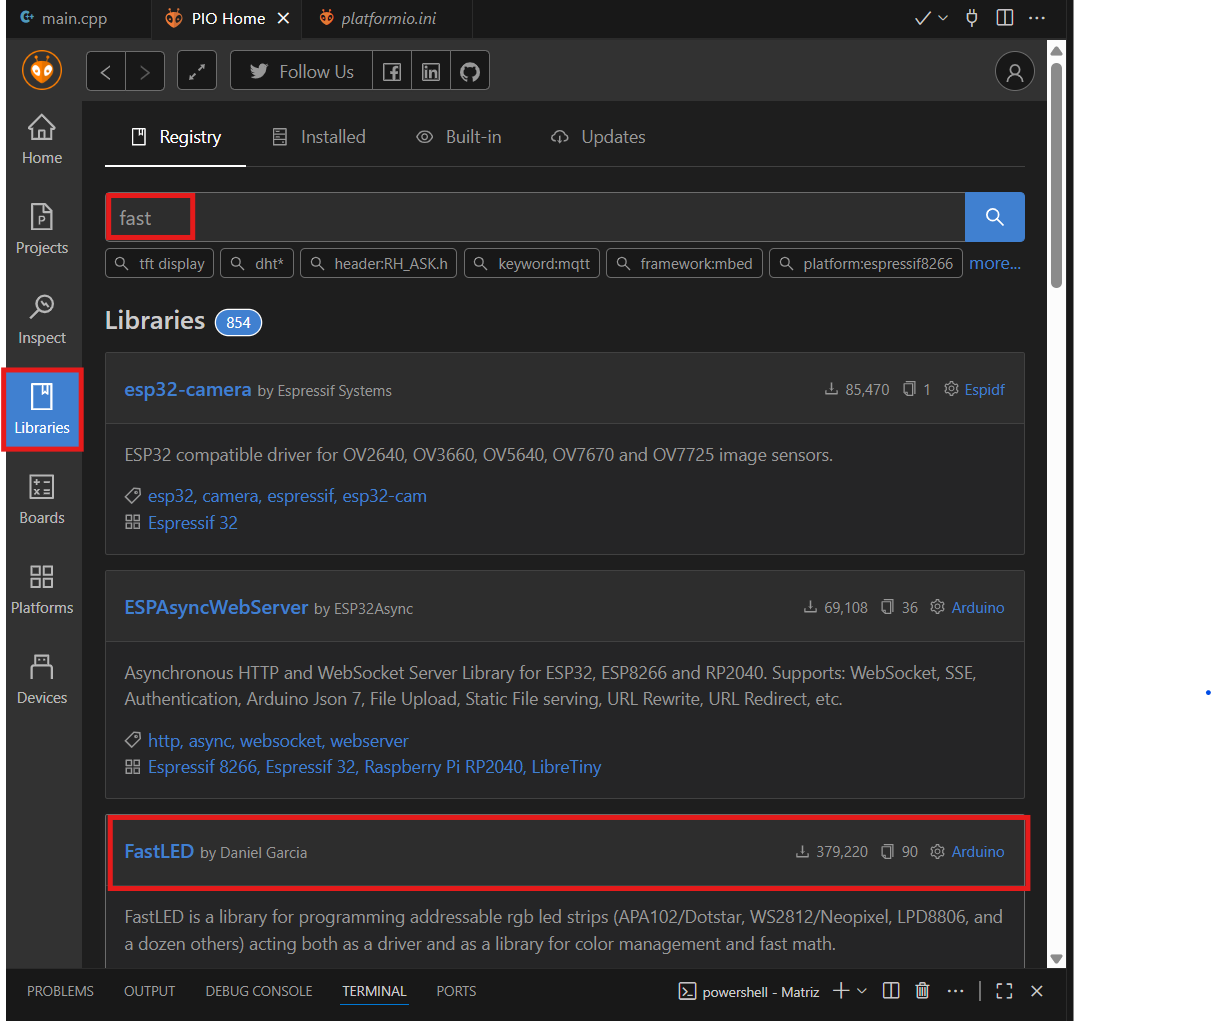
\includegraphics[width=0.75\textwidth]{Platformio/librerias_1.png}
  \caption{Instalación de la librería \texttt{FastLED} desde el gestor de librerías de PlatformIO.}
\end{figure}

\begin{figure}[H]
  \centering
  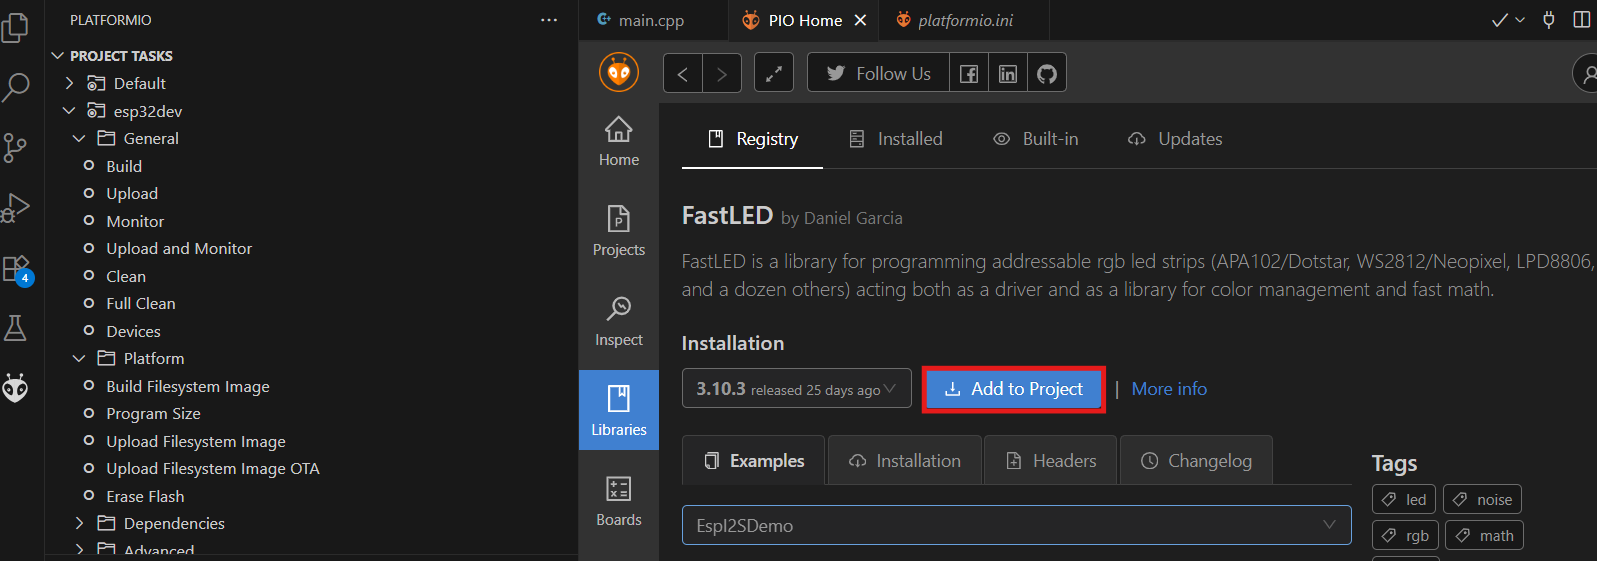
\includegraphics[width=0.75\textwidth]{Platformio/librerias_2.png}
  \caption{Instalación de la librería \texttt{FastLED} desde el gestor de librerías de PlatformIO.}
\end{figure}

\subsubsection{Método 2: agregando la dependencia en \texttt{platformio.ini}}

Otra forma de instalar la librería es editando manualmente el archivo de configuración \texttt{platformio.ini} del proyecto, añadiendo la línea:

\newpage

\begin{lstlisting}[language=c,caption={Configuracion de librerias en platformio.ini}]
[env:esp32dev]
platform = espressif32
board = esp32dev
framework = arduino
lib_deps = FastLED
\end{lstlisting}

Al guardar el archivo, PlatformIO descargará automáticamente la librería la próxima vez que se compile el proyecto.

\begin{figure}[H]
  \centering
  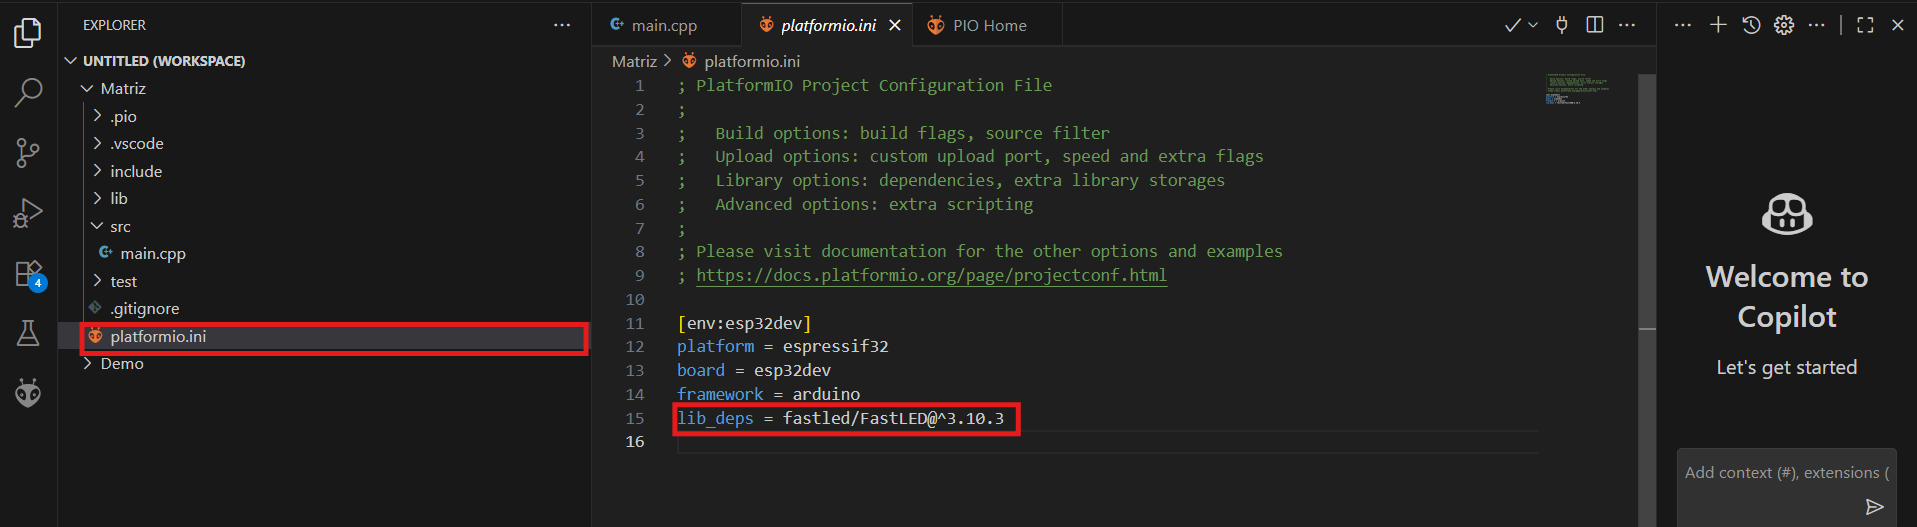
\includegraphics[width=0.75\textwidth]{Platformio/forma_2.png}
  \caption{Ejemplo de archivo \texttt{platformio.ini} con la dependencia de \texttt{FastLED} añadida.}
\end{figure}

\subsection{Explicación del código por bloques}



\subsubsection{Código completo}

\begin{lstlisting}[language=C++, caption={Código completo para la matriz LED 16x16 con ESP32 y FastLED}]
#include <Arduino.h>
// Matriz 16x16 WS2812 con ESP32 (FastLED)
// Data: GPIO4 por defecto. Cambia según tu conexión.

#include <FastLED.h>

#define MATRIX_WIDTH 16
#define MATRIX_HEIGHT 16
#define NUM_LEDS (MATRIX_WIDTH * MATRIX_HEIGHT)
#define DATA_PIN 4        // pin de datos al primer LED
#define BUTTON_PIN 2      // cambiar si usas diferente
#define BRIGHTNESS 120    // reducción para no sobrecargar la fuente

CRGB leds[NUM_LEDS];

// --- Configuración de modos / botones
volatile uint8_t mode = 0;
const uint8_t MODES = 5;
unsigned long lastButtonMillis = 0;
const unsigned long debounce = 200;

// --- Variables de control de modos (para reiniciar estado al cambiar de modo)
uint8_t prevMode = 255;
bool showHolaDone = false;

// --- Mapeo XY para matriz serpentina (zig-zag)
inline uint16_t XY(uint8_t x, uint8_t y){
  if(x >= MATRIX_WIDTH || y >= MATRIX_HEIGHT) return 0;
  if(y % 2 == 0) {
    return (y * MATRIX_WIDTH) + (MATRIX_WIDTH - 1 - x);
  } else {
    return (y * MATRIX_WIDTH) + x;
  }
}

// ----------------- Fuente 5x7 (A-Z + espacio) -----------------
const uint8_t font5x7[][5] = {
  {0x7C,0x12,0x11,0x12,0x7C}, // A
  {0x7F,0x49,0x49,0x49,0x36}, // B
  {0x3E,0x41,0x41,0x41,0x22}, // C
  {0x7F,0x41,0x41,0x22,0x1C}, // D
  {0x7F,0x49,0x49,0x49,0x41}, // E
  {0x7F,0x09,0x09,0x09,0x01}, // F
  {0x3E,0x41,0x49,0x49,0x7A}, // G
  {0x7F,0x08,0x08,0x08,0x7F}, // H
  {0x00,0x41,0x7F,0x41,0x00}, // I
  {0x20,0x40,0x41,0x3F,0x01}, // J
  {0x7F,0x08,0x14,0x22,0x41}, // K
  {0x7F,0x40,0x40,0x40,0x40}, // L
  {0x7F,0x02,0x0C,0x02,0x7F}, // M
  {0x7F,0x04,0x08,0x10,0x7F}, // N
  {0x3E,0x41,0x41,0x41,0x3E}, // O
  {0x7F,0x09,0x09,0x09,0x06}, // P
  {0x3E,0x41,0x51,0x21,0x5E}, // Q
  {0x7F,0x09,0x19,0x29,0x46}, // R
  {0x46,0x49,0x49,0x49,0x31}, // S
  {0x01,0x01,0x7F,0x01,0x01}, // T
  {0x3F,0x40,0x40,0x40,0x3F}, // U
  {0x1F,0x20,0x40,0x20,0x1F}, // V
  {0x3F,0x40,0x38,0x40,0x3F}, // W
  {0x63,0x14,0x08,0x14,0x63}, // X
  {0x07,0x08,0x70,0x08,0x07}, // Y
  {0x61,0x51,0x49,0x45,0x43}, // Z
  {0x00,0x00,0x00,0x00,0x00}  // espacio (index 26)
};

inline int fontIndex(char c){
  if(c >= 'A' && c <= 'Z') return c - 'A';
  if(c == ' ') return 26;
  return 26;
}

// --- Efectos originales (sin tocar mucho)
void rainbowChase(uint8_t wait){
  static uint8_t startHue = 0;
  for(uint8_t y=0;y<MATRIX_HEIGHT;y++){
    for(uint8_t x=0;x<MATRIX_WIDTH;x++){
      uint16_t i = XY(x,y);
      uint8_t hue = startHue + (x*8) + (y*4);
      leds[i] = CHSV(hue, 200, 255);
    }
  }
  startHue += 1;
  FastLED.show();
  delay(wait);
}

void plasma(uint8_t t){
  static uint16_t count = 0;
  for(uint8_t y=0;y<MATRIX_HEIGHT;y++){
    for(uint8_t x=0;x<MATRIX_WIDTH;x++){
      float v = sinf((x+count)/4.0f) + sinf((y-count)/3.0f) + sinf((x+y+count)/5.0f);
      uint8_t hue = (uint8_t)map((int)((v+3.0f)*40.0f), 0, 240, 0, 255);
      leds[XY(x,y)] = CHSV(hue, 220, 200);
    }
  }
  count += t;
  FastLED.show();
  delay(20);
}

void fireworks(){
  static CRGB fade[NUM_LEDS];
  // decay: 250 es rápido, 200 es más lento (más fácil de ver)
  const uint8_t decay = 200;
  for(int i=0;i<NUM_LEDS;i++){
    fade[i].nscale8(decay); // reduce brillo de cada frame
  }

  const int spawnRate = 20; // prueba con 20 (más frecuente). Pon 5 para muchas.
  if(random(0, spawnRate) == 0){
    int cx = random(2, MATRIX_WIDTH - 2);
    int cy = random(2, MATRIX_HEIGHT - 2);
    CRGB color = CHSV(random8(), 255, 255);
    for(int dx = -2; dx <= 2; dx++){
      for(int dy = -2; dy <= 2; dy++){
        int x = cx + dx;
        int y = cy + dy;
        if(x >= 0 && x < MATRIX_WIDTH && y >= 0 && y < MATRIX_HEIGHT){
          float dist = sqrtf((float)(dx*dx + dy*dy));
          int bright = 255 - int(dist * 90.0f);
          if(bright > 0){
            CRGB scaled = color;
            scaled.nscale8((uint8_t)bright);
            fade[XY(x,y)] += scaled;
          }
        }
      }
    }
  }

  for(int i=0;i<NUM_LEDS;i++) leds[i] = fade[i];
  FastLED.show();
  delay(35);
}

void checkerboard(uint8_t t){
  for(uint8_t y=0;y<MATRIX_HEIGHT;y++){
    for(uint8_t x=0;x<MATRIX_WIDTH;x++){
      bool on = ((x/2 + y/2 + (t/10)) % 2) == 0;
      uint16_t idx = XY(x,y);
      if(on){
        leds[idx] = CHSV( (uint8_t)(160 + (x*3)), 200, 255 );
      } else {
        leds[idx] = CRGB::Black;
      }
    }
  }
  FastLED.show();
  delay(40);
}

// ----------------- Funciones de texto y scroll -----------------
void clearMatrix(){
  for(int i=0;i<NUM_LEDS;i++) leds[i] = CRGB::Black;
}

inline void drawPixelSafe(int x, int y, CRGB color){
  if(x < 0 || x >= MATRIX_WIDTH || y < 0 || y >= MATRIX_HEIGHT) return;
  leds[XY(x,y)] = color;
}

void drawTextAt(int x0, const char* text, CRGB color){
  int x = x0;
  for(size_t i=0; text[i] != '\0'; ++i){
    char c = text[i];
    if(c >= 'a' && c <= 'z') c = c - 'a' + 'A';
    int idx = fontIndex(c);
    const uint8_t *glyph = font5x7[idx];
    for(int col=0; col<5; ++col){
      uint8_t columnBits = glyph[col];
      for(int row=0; row<7; ++row){
        if(columnBits & (1<<row)){
          int y = row + (MATRIX_HEIGHT - 7)/2;
          drawPixelSafe(x + col, y, color);
        }
      }
    }
    x += 6; // 5 columnas + 1 columna de espacio
  }
}

void scrollMessage(const char* text, uint8_t speed, CHSV colorHSV){
  int len = strlen(text);
  int totalCols = len * 6;
  uint8_t *cols = (uint8_t*)malloc(totalCols);
  if(!cols) return;
  int colIdx = 0;
  for(int i=0;i<len;i++){
    char c = text[i];
    if(c >= 'a' && c <= 'z') c = c - 'a' + 'A';
    int fi = fontIndex(c);
    const uint8_t *g = font5x7[fi];
    for(int ccol=0; ccol<5; ++ccol){
      cols[colIdx++] = g[ccol];
    }
    cols[colIdx++] = 0x00;
  }

  int scrollRange = totalCols + MATRIX_WIDTH;
  for(int off = 0; off < scrollRange; ++off){
    clearMatrix();
    for(int x=0; x < MATRIX_WIDTH; ++x){
      int sourceCol = off + x - MATRIX_WIDTH;
      if(sourceCol >= 0 && sourceCol < totalCols){
        uint8_t columnBits = cols[sourceCol];
        for(int row=0; row<7; ++row){
          if(columnBits & (1<<row)){
            int y = row + (MATRIX_HEIGHT - 7)/2;
            drawPixelSafe(x, y, colorHSV);
          }
        }
      }
    }
    FastLED.show();
    delay(speed);
  }

  free(cols);
}

void showHola(unsigned long duration = 2000){
  const char *msg = "HOLA";
  int len = strlen(msg);
  int width = len * 6 - 1;
  int x0 = (MATRIX_WIDTH - width) / 2;
  if(x0 < 0) x0 = 0;
  clearMatrix();
  drawTextAt(x0, msg, CHSV(160, 200, 255));
  FastLED.show();
  delay(duration);
}

// ----------------- Interrupción de botón (secuencial de modos) -----------------
void IRAM_ATTR handleButton(){
  unsigned long now = millis();
  if(now - lastButtonMillis < debounce) return;
  lastButtonMillis = now;
  mode = (mode + 1) % MODES;
}

// ----------------- Setup / Loop -----------------
void setup(){
  Serial.begin(115200);
  delay(100);
  FastLED.addLeds<WS2812, DATA_PIN, GRB>(leds, NUM_LEDS).setCorrection(TypicalLEDStrip);
  FastLED.setBrightness(BRIGHTNESS);
  pinMode(BUTTON_PIN, INPUT_PULLUP);
  attachInterrupt(digitalPinToInterrupt(BUTTON_PIN), handleButton, FALLING);
  randomSeed(analogRead(36));
  clearMatrix();
  FastLED.show();
}

void loop(){
  if(prevMode != mode){
    prevMode = mode;
    showHolaDone = false;
  }

  switch(mode){
    case 0:
      rainbowChase(20);
      break;
    case 1:
      plasma(1);
      break;
    case 2:
      fireworks();
      break;
    case 3:
      checkerboard(millis()/50);
      break;
    case 4:
      scrollMessage("UPS CUENCA", 60, CHSV(0, 0, 255));
      break;
    default:
      mode = 0;
  }
}
\end{lstlisting}

\subsubsection{Inclusiones y definiciones principales}

\begin{lstlisting}[language=C++, caption={Inclusiones y macros principales}]
#include <Arduino.h>
#include <FastLED.h>

#define MATRIX_WIDTH 16
#define MATRIX_HEIGHT 16
#define NUM_LEDS (MATRIX_WIDTH * MATRIX_HEIGHT)
#define DATA_PIN 4
#define BUTTON_PIN 2
#define BRIGHTNESS 120
\end{lstlisting}

Este bloque carga las librerías esenciales y define parámetros constantes: tamaño de la matriz, número total de LEDs, pines de datos y del botón, y el brillo máximo. Las macros facilitan cambiar dimensiones o pines en un solo lugar sin buscar en todo el código. El valor de brillo se reduce para limitar la corriente consumida por la matriz.

\newpage

\subsubsection{Declaración del buffer y variables de control}

\begin{lstlisting}[language=C++, caption={Buffer de LEDs y variables de control}]
CRGB leds[NUM_LEDS];

volatile uint8_t mode = 0;
const uint8_t MODES = 5;
unsigned long lastButtonMillis = 0;
const unsigned long debounce = 200;

uint8_t prevMode = 255;
bool showHolaDone = false;
\end{lstlisting}

Aquí se reserva el arreglo que representa cada LED en memoria (formato CRGB). También se declaran variables que controlan el modo actual, el número total de modos, y el mecanismo de debounce para evitar lecturas múltiples del botón por rebote. `prevMode` y `showHolaDone` sirven para detectar cambios de modo y manejar acciones que sólo deben ejecutarse al entrar en un modo.

\subsubsection{Mapeo XY (serpentina)}

\begin{lstlisting}[language=C++, caption={Función de mapeo XY para matriz serpentina}]
inline uint16_t XY(uint8_t x, uint8_t y){
  if(x >= MATRIX_WIDTH || y >= MATRIX_HEIGHT) return 0;
  if(y % 2 == 0) {
    return (y * MATRIX_WIDTH) + (MATRIX_WIDTH - 1 - x);
  } else {
    return (y * MATRIX_WIDTH) + x;
  }
}
\end{lstlisting}

Convierte coordenadas (x,y) en el índice lineal usado por el buffer `leds[]`, corrigiendo la disposición física serpentina (zig-zag). Si la fila es par, se invierte el orden horizontal para coincidir con el cableado típico de matrices WS2812; si la fila es impar, se usa el orden natural. La validación inicial evita accesos fuera de rango.

\newpage

\subsubsection{Fuente 5x7 y helper de índice}

\begin{lstlisting}[language=C++, caption={Fuente 5x7 y función auxiliar}]
const uint8_t font5x7[][5] = {
  {0x7C,0x12,0x11,0x12,0x7C}, // A
  {0x7F,0x49,0x49,0x49,0x36}, // B
  ...
  {0x00,0x00,0x00,0x00,0x00}  // espacio
};

inline int fontIndex(char c){
  if(c >= 'A' && c <= 'Z') return c - 'A';
  if(c == ' ') return 26;
  return 26;
}
\end{lstlisting}

Contiene las columnas de bits por carácter para una fuente de 5×7. Cada byte representa una columna vertical de 7 píxeles; cinco bytes forman un glifo. La función auxiliar mapea un carácter ASCII (A–Z o espacio) al índice correcto del arreglo. Si el carácter no se reconoce, se devuelve el índice del espacio.

\subsubsection{Efecto: rainbowChase}

\begin{lstlisting}[language=C++, caption={Efecto rainbowChase}]
void rainbowChase(uint8_t wait){
  static uint8_t startHue = 0;
  for(uint8_t y=0;y<MATRIX_HEIGHT;y++){
    for(uint8_t x=0;x<MATRIX_WIDTH;x++){
      uint16_t i = XY(x,y);
      uint8_t hue = startHue + (x*8) + (y*4);
      leds[i] = CHSV(hue, 200, 255);
    }
  }
  startHue += 1;
  FastLED.show();
  delay(wait);
}
\end{lstlisting}

Genera un gradiente de color en modo HSV donde el tono depende de la posición x,y y de un desplazamiento `startHue` que cambia en el tiempo para animar el arcoíris. `CHSV` simplifica la manipulación de color y `FastLED.show()` actualiza físicamente la matriz. El parámetro `wait` regula la velocidad del efecto.

\subsubsection{Efecto: plasma}

\begin{lstlisting}[language=C++, caption={Efecto plasma}]
void plasma(uint8_t t){
  static uint16_t count = 0;
  for(uint8_t y=0;y<MATRIX_HEIGHT;y++){
    for(uint8_t x=0;x<MATRIX_WIDTH;x++){
      float v = sinf((x+count)/4.0f) + sinf((y-count)/3.0f) + sinf((x+y+count)/5.0f);
      uint8_t hue = (uint8_t)map((int)((v+3.0f)*40.0f), 0, 240, 0, 255);
      leds[XY(x,y)] = CHSV(hue, 220, 200);
    }
  }
  count += t;
  FastLED.show();
  delay(20);
}
\end{lstlisting}

Crea un efecto ondulante combinando varias funciones seno para obtener variaciones suaves en el valor `v`. Ese valor se mapea a un tono HSV que produce las transiciones de color tipo plasma. La variable `count` avanza con el tiempo para desplazar la animación; el parámetro `t` controla la velocidad de avance.

\subsubsection{Efecto: fireworks}

\begin{lstlisting}[language=C++, caption={Efecto fireworks}]
void fireworks(){
  static CRGB fade[NUM_LEDS];
  const uint8_t decay = 200;
  for(int i=0;i<NUM_LEDS;i++){
    fade[i].nscale8(decay);
  }

  const int spawnRate = 20;
  if(random(0, spawnRate) == 0){
    int cx = random(2, MATRIX_WIDTH - 2);
    int cy = random(2, MATRIX_HEIGHT - 2);
    CRGB color = CHSV(random8(), 255, 255);
    for(int dx = -2; dx <= 2; dx++){
      for(int dy = -2; dy <= 2; dy++){
        int x = cx + dx;
        int y = cy + dy;
        if(x >= 0 && x < MATRIX_WIDTH && y >= 0 && y < MATRIX_HEIGHT){
          float dist = sqrtf((float)(dx*dx + dy*dy));
          int bright = 255 - int(dist * 90.0f);
          if(bright > 0){
            CRGB scaled = color;
            scaled.nscale8((uint8_t)bright);
            fade[XY(x,y)] += scaled;
          }
        }
      }
    }
  }

  for(int i=0;i<NUM_LEDS;i++) leds[i] = fade[i];
  FastLED.show();
  delay(35);
}
\end{lstlisting}

Mantiene un buffer `fade[]` que decae cada frame (escala hacia abajo el brillo). Ocasionalmente se genera una explosión en una posición aleatoria, pintando píxeles en un radio y sumando su contribución al buffer. El decaimiento hace que las explosiones se atenúen con el tiempo, creando el efecto de fuegos artificiales.

\subsubsection{Efecto: checkerboard}

\begin{lstlisting}[language=C++, caption={Efecto checkerboard}]
void checkerboard(uint8_t t){
  for(uint8_t y=0;y<MATRIX_HEIGHT;y++){
    for(uint8_t x=0;x<MATRIX_WIDTH;x++){
      bool on = ((x/2 + y/2 + (t/10)) % 2) == 0;
      uint16_t idx = XY(x,y);
      if(on){
        leds[idx] = CHSV( (uint8_t)(160 + (x*3)), 200, 255 );
      } else {
        leds[idx] = CRGB::Black;
      }
    }
  }
  FastLED.show();
  delay(40);
}
\end{lstlisting}

Dibuja un tablero de cuadros alternados donde el patrón se desplaza en el tiempo (la expresión `(t/10)` añade animación). La condición `on` decide si una celda está encendida; el color varía ligeramente por columna para dar dinamismo.

\subsubsection{Utilidades de dibujo y texto}

\begin{lstlisting}[language=C++, caption={Funciones clearMatrix, drawPixelSafe, drawTextAt}]
void clearMatrix(){
  for(int i=0;i<NUM_LEDS;i++) leds[i] = CRGB::Black;
}
inline void drawPixelSafe(int x, int y, CRGB color){
  if(x < 0 || x >= MATRIX_WIDTH || y < 0 || y >= MATRIX_HEIGHT) return;
  leds[XY(x,y)] = color;
}
void drawTextAt(int x0, const char* text, CRGB color){
  int x = x0;
  for(size_t i=0; text[i] != '\0'; ++i){
    char c = text[i];
    if(c >= 'a' && c <= 'z') c = c - 'a' + 'A';
    int idx = fontIndex(c);
    const uint8_t *glyph = font5x7[idx];
    for(int col=0; col<5; ++col){
      uint8_t columnBits = glyph[col];
      for(int row=0; row<7; ++row){
        if(columnBits & (1<<row)){
          int y = row + (MATRIX_HEIGHT - 7)/2;
          drawPixelSafe(x + col, y, color);
        }
      }
    }
    x += 6;
  }
}
\end{lstlisting}

`clearMatrix()` pone todos los LEDs a negro. `drawPixelSafe()` escribe un pixel solo si está dentro de los límites, evitando accesos inválidos. `drawTextAt()` recorre cada carácter, extrae su glifo en columnas y pinta las columnas en la posición horizontal indicada; hace conversión a mayúsculas para simplificar el mapeo con la tabla de fuente.

\subsubsection{Scroll de texto}

\begin{lstlisting}[language=C++, caption={Función scrollMessage}]
void scrollMessage(const char* text, uint8_t speed, CHSV colorHSV){
  int len = strlen(text);
  int totalCols = len * 6;
  uint8_t *cols = (uint8_t*)malloc(totalCols);
  if(!cols) return;
  int colIdx = 0;
  for(int i=0;i<len;i++){
    char c = text[i];
    if(c >= 'a' && c <= 'z') c = c - 'a' + 'A';
    int fi = fontIndex(c);
    const uint8_t *g = font5x7[fi];
    for(int ccol=0; ccol<5; ++ccol){
      cols[colIdx++] = g[ccol];
    }
    cols[colIdx++] = 0x00;
  }

  int scrollRange = totalCols + MATRIX_WIDTH;
  for(int off = 0; off < scrollRange; ++off){
    clearMatrix();
    for(int x=0; x < MATRIX_WIDTH; ++x){
      int sourceCol = off + x - MATRIX_WIDTH;
      if(sourceCol >= 0 && sourceCol < totalCols){
        uint8_t columnBits = cols[sourceCol];
        for(int row=0; row<7; ++row){
          if(columnBits & (1<<row)){
            int y = row + (MATRIX_HEIGHT - 7)/2;
            drawPixelSafe(x, y, colorHSV);
          }
        }
      }
    }
    FastLED.show();
    delay(speed);
  }

  free(cols);
}
\end{lstlisting}

Construye un buffer de columnas (5 columnas por carácter + 1 columna vacía) y recorre ese buffer desplazándolo sobre la matriz. Para cada desplazamiento se limpia la matriz, se calculan las columnas visibles y se pintan los píxeles según los bits de cada columna. `speed` controla el retardo entre pasos y, por tanto, la velocidad del scroll. Se usa `malloc` y `free` para el buffer; en sistemas con memoria limitada, considerar usar un buffer estático o streaming para evitar fragmentación.

\subsubsection{Mensaje de bienvenida}

\begin{lstlisting}[language=C++, caption={Función showHola}]
void showHola(unsigned long duration = 2000){
  const char *msg = "HOLA";
  int len = strlen(msg);
  int width = len * 6 - 1;
  int x0 = (MATRIX_WIDTH - width) / 2;
  if(x0 < 0) x0 = 0;
  clearMatrix();
  drawTextAt(x0, msg, CHSV(160, 200, 255));
  FastLED.show();
  delay(duration);
}
\end{lstlisting}

Centra el texto "HOLA" en la matriz calculando el ancho en columnas y usando `drawTextAt()` para dibujarlo. Se muestra durante el tiempo indicado por `duration`, útil como introducción al iniciar o al cambiar de modo.

\newpage

\subsubsection{ISR del botón}

\begin{lstlisting}[language=C++, caption={Rutina de interrupción handleButton}]
void IRAM_ATTR handleButton(){
  unsigned long now = millis();
  if(now - lastButtonMillis < debounce) return;
  lastButtonMillis = now;
  mode = (mode + 1) % MODES;
}
\end{lstlisting}

Rutina que se ejecuta en respuesta a la señal del botón. Implementa debounce temporal (ignorando pulsos más rápidos que debounce) y avanza la variable mode de forma cíclica. La etiqueta IRAM\_ATTR sugiere que la función se coloque en la IRAM del ESP32 para una respuesta más fiable en interrupciones.

\subsubsection{setup()}

\begin{lstlisting}[language=C++, caption={Función setup}]
void setup(){
  Serial.begin(115200);
  delay(100);
  FastLED.addLeds<WS2812, DATA_PIN, GRB>(leds, NUM_LEDS).setCorrection(TypicalLEDStrip);
  FastLED.setBrightness(BRIGHTNESS);
  pinMode(BUTTON_PIN, INPUT_PULLUP);
  attachInterrupt(digitalPinToInterrupt(BUTTON_PIN), handleButton, FALLING);
  randomSeed(analogRead(36));
  clearMatrix();
  FastLED.show();
}
\end{lstlisting}

Inicializa la comunicación serial, configura la librería FastLED con el tipo de LEDs y el buffer, ajusta brillo, configura el pin del botón con pull-up interno y enlaza la interrupción al pin. También inicializa la semilla aleatoria y limpia la matriz antes de comenzar.

\newpage

\subsubsection{loop()}

\begin{lstlisting}[language=C++, caption={Bucle principal loop}]
void loop(){
  if(prevMode != mode){
    prevMode = mode;
    showHolaDone = false;
  }

  switch(mode){
    case 0:
      rainbowChase(20);
      break;
    case 1:
      plasma(1);
      break;
    case 2:
      fireworks();
      break;
    case 3:
      checkerboard(millis()/50);
      break;
    case 4:
      scrollMessage("UPS CUENCA", 60, CHSV(0, 0, 255));
      break;
    default:
      mode = 0;
  }
}
\end{lstlisting}

Bucle principal que detecta cambios de modo para poder reiniciar estados y luego ejecuta el efecto correspondiente según `mode`. Cada caso llama a la función que dibuja y actualiza la matriz; el flujo permanece en esa función hasta que ésta retorna y el bucle se vuelve a ejecutar (el botón puede cambiar `mode` desde la ISR en cualquier momento).


\section{Carga del programa en la placa y verificación}

Esta sección explica paso a paso cómo compilar el proyecto en PlatformIO (VSCode) y cargarlo en la placa ESP32, además de cómo verificar que el programa se ejecuta correctamente mediante pruebas en la matriz LED y la consola serial.

\subsection{Comprobaciones previas}
Antes de compilar y cargar:
\begin{itemize}
  \item Asegurar que la placa ESP32 está conectada al ordenador por USB y que la masa (GND) comparte referencia con la fuente de la matriz LED si ésta tiene alimentación externa.
  \item Revisar el archivo \texttt{platformio.ini} y confirmar que la seccion \texttt{env} usa la placa correcta (por ejemplo, \texttt{board = esp32dev}) y el framework \texttt{arduino}.
  \item Instalar drivers USB si el sistema operativo los solicita (por ejemplo CP210x o CH340, según la placa).
  \item Verificar que \texttt{FastLED} está añadida en \texttt{lib\_deps} o instalada desde el gestor de librerías de PlatformIO.
\end{itemize}

\begin{lstlisting}[language=ini,caption={Ejemplo mínimo de \texttt{platformio.ini}}]
[env:esp32dev]
platform = espressif32
board = esp32dev
framework = arduino
monitor_speed = 115200
lib_deps =
  FastLED
build_flags = 
  ; opciones adicionales si se requieren
\end{lstlisting}

\subsection{Compilar el proyecto (Build)}

\begin{enumerate}
  \item Abrir el proyecto en VSCode y seleccionar el icono de PlatformIO en la barra lateral.
  \item Pulsar el botón \textbf{Build} (icono de check / "Build") o usar el atajo en la barra inferior de PlatformIO.
  \item Observar la consola de salida: PlatformIO descargará dependencias (si es la primera vez) y compilará el proyecto.  
\end{enumerate}

\begin{figure}[H]
  \centering
  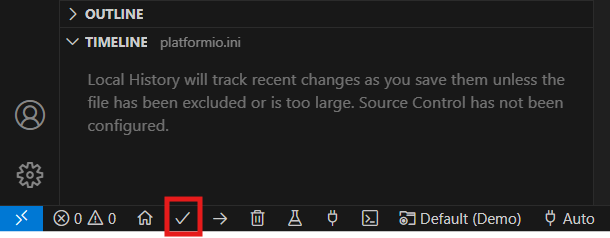
\includegraphics[width=0.75\textwidth]{Platformio/verify.png}
  \caption{Compilación del proyecto en PlatformIO — salida en la pestaña \textit{Terminal / Output}.}
\end{figure}

Si la compilación falla, revisar errores en la consola. Los mensajes habituales incluyen librerías faltantes, errores de sintaxis o definiciones de pines inconsistentes.

\subsection{Seleccionar puerto serie y subir (Upload)}

\begin{enumerate}
  \item Con la placa conectada, identificar el puerto COM (Windows) o \texttt{/dev/ttyUSB*} (Linux/macOS). En VSCode → PlatformIO → \textbf{Devices} suele aparecer el puerto detectado.
  \item Si el puerto no aparece, instalar el driver USB correcto o probar con otro cable USB (muchos cables son solo de carga).
  \item Pulsar el botón \textbf{Upload} (icono de flecha) en PlatformIO o usar el comando \texttt{PlatformIO: Upload} desde la paleta de comandos.
  \item Observar la salida: PlatformIO compilará (si es necesario) y ejecutará el proceso de subida (esptool). Esperar a que indique \texttt{SUCCESS} o \texttt{DONE}.
\end{enumerate}

\begin{figure}[H]
  \centering
  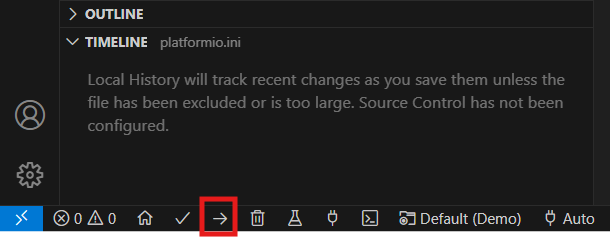
\includegraphics[width=0.75\textwidth]{Platformio/cargar.png}
  \caption{Proceso de subida (Upload) en PlatformIO.}
\end{figure}

\section{Resultados}

En esta sección se documenta el funcionamiento del firmware ejecutado en el ESP32 controlando la matriz WS2812 16\(\times\)16. Se incluyen fotografías y capturas de pantalla tomadas directamente de la matriz en funcionamiento. Para cada imagen se describe el modo probado y el comportamiento esperado.

\begin{figure}[H]
  \centering
  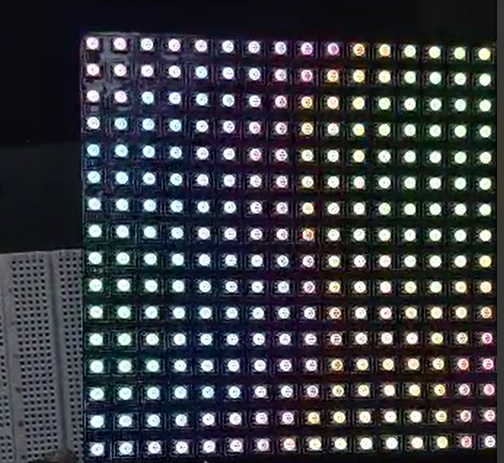
\includegraphics[width=0.7\textwidth]{Resultados/rainbow.png}
  \caption{Modo 0 — \textit{rainbowChase}: se espera un gradiente arcoíris que recorre la matriz; los tonos deben cambiar suavemente horizontal y verticalmente.}
\end{figure}


\begin{figure}[H]
  \centering
  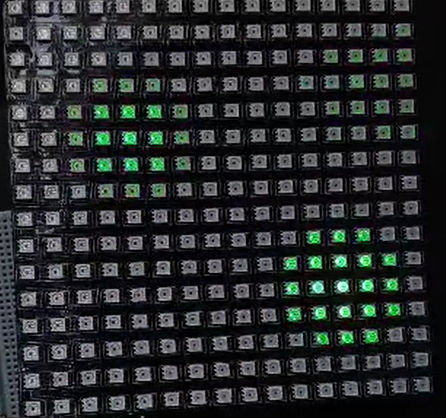
\includegraphics[width=0.7\textwidth]{Resultados/fireworks.png}
  \caption{Modo 2 — \textit{fireworks}: explosiones puntuales con atenuación gradual; documentar al menos una explosión y su decaimiento.}
\end{figure}

\begin{figure}[H]
  \centering
  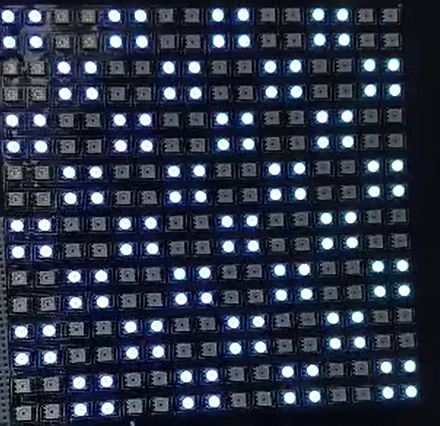
\includegraphics[width=0.7\textwidth]{Resultados/chess.png}
  \caption{Modo 3 — \textit{checkerboard}: patrón de tablero en movimiento; verificar alternancia de cuadros y desplazamiento temporal.}
\end{figure}

\begin{figure}[H]
  \centering
  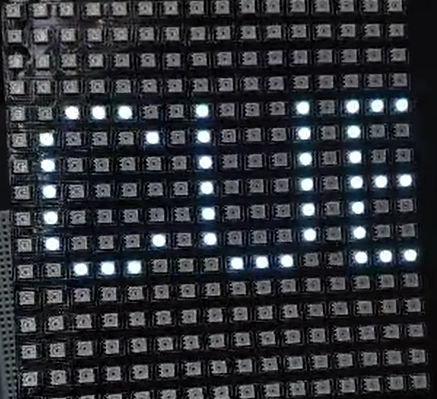
\includegraphics[width=0.7\textwidth]{Resultados/scroll.png}
  \caption{Modo 4 — \textit{scrollMessage}: texto desplazándose (ej.: ``UPS CUENCA''); capturar una secuencia de 3–5 frames que muestre el texto entrando, centrado y saliendo.}
\end{figure}


\end{document}
